\documentclass{beamer}
%\documentclass[handout]{beamer}

%\setbeamertemplate{theorems}[numbered]
\setbeamertemplate{theorems}[ams style]
\setbeamertemplate{caption}[numbered]

\usepackage{lmodern} % get rid of warnings
\usepackage{caption} % improved spacing between figure and caption

\DeclareCaptionLabelSeparator{horse}{:\quad} % change according to your needs
\captionsetup{
	labelsep = horse,
	figureposition = bottom
} 

%\usepackage[utf8]{inputenc}
\usepackage[T1]{fontenc}
\usepackage[english]{babel}

\usepackage{amsfonts}
\usepackage{amsmath}
\usepackage{amssymb}
\usepackage{amsthm}
% \usepackage[frenchstyle]{mathalpha}
% \usepackage[OMLmathsfit]{isomath}
\usepackage{graphicx}
\usepackage{color} % for ps_tex inclusions
\usepackage{fmtcount} % th, e.g. \ordinalnum{4}
\usepackage{algorithm, algorithmic} % algorithms
\usepackage{tikz}
\usetikzlibrary{bayesnet,calc,tikzmark}
\usetikzlibrary{shapes.geometric}
\tikzset{  net/.style={draw,trapezium,trapezium angle=65,shape border rotate=270} }
\tikzset{  rnn/.style={draw,rectangle} }
\usepackage{xr}
\usepackage{hyperref}
\externaldocument[notes-]{notes}
\usetheme{Madrid}
\usecolortheme{seagull}

\newcommand{\itb}{\item[$\bullet$]}
\newcommand{\dps}{\displaystyle}

\def\<{{\guillemotleft}}
\def\>{{\guillemotright}}

\def\vs1{\vspace{1mm}}
\def\v3{\vspace{3mm}}

\newcommand{\II}{\,\mbox{I\hskip -0.600em 1}}

\newcommand{\BSX}{{\boldsymbol X}}
\newcommand{\BSY}{{\boldsymbol Y}}
\newcommand{\BSZ}{{\boldsymbol Z}}

\newcommand{\bsx}{{\boldsymbol x}}
\newcommand{\bsy}{{\boldsymbol y}}
\newcommand{\bsz}{{\boldsymbol z}}

\newcommand{\bsalpha}{{\boldsymbol \alpha}}

\newcommand{\MA}{{\mathcal A}}
\newcommand{\MB}{{\mathcal B}}
\newcommand{\MC}{{\mathcal C}}
\newcommand{\MD}{{\mathcal D}}
\newcommand{\ME}{{\mathcal E}}
\newcommand{\MF}{{\mathcal F}}
\newcommand{\MG}{{\mathcal G}}
\newcommand{\MK}{{\mathcal K}}
\newcommand{\MM}{{\mathcal M}}
\newcommand{\MN}{{\mathcal N}}
\newcommand{\MO}{{\mathcal O}}
\newcommand{\MQ}{{\mathcal Q}}
\newcommand{\MS}{{\mathcal S}}
\newcommand{\MT}{{\mathcal T}}
\newcommand{\MU}{{\mathcal U}}
\newcommand{\MV}{{\mathcal V}}
\newcommand{\MX}{{\mathcal X}}

\newcommand{\TY}{{\tilde Y}}

\newcommand{\NN}{\ensuremath{\mathbb{N}}}
\newcommand{\RR}{\ensuremath{\mathbb{R}}}

\newcommand{\card}{\mbox{card}}
\newcommand{\pa}{\mbox{pa}}

\newcommand{\De}{\mbox{De}}
\newcommand{\Nd}{\mbox{Nd}}
\newcommand{\Ne}{\mbox{Ne}}

\newcommand{\indep}{\perp\!\!\!\perp}
\newcommand{\condindep}[3]{#1 \indep #2 \vert #3}
\newcommand{\condindepP}[4]{#1 \indep_{#4} #2 \vert #3}
\newcommand{\ts}[3]{#1_{#2}^{#3}}
\newcommand{\set}[1]{\{#1\}}

\newcommand{\myth}[1]{#1^{\mbox{\scriptsize{th}}}}


\newcommand{\myarray}[2]{\left(\begin{array}{#1}#2\end{array}\right)}

\title[LPC]{Learning, Probabilities, and Causality}

\subtitle{Chapter VI - Variational Autoencoders (VAE)} % (optional)

\author[Xavi]{Xavier Alameda-Pineda}
% - Use the \inst{?} command only if the authors have different
%   affiliation.

\institute{}

\date{}

\makeatother
\setbeamertemplate{footline}
{
  \leavevmode%
%   \hbox{%
%   \begin{beamercolorbox}[wd=.4\paperwidth,ht=2.25ex,dp=1ex,center]{author in head/foot}%
%     \usebeamerfont{author in head/foot}\insertshortauthor
%   \end{beamercolorbox}%
%   \begin{beamercolorbox}[wd=.6\paperwidth,ht=2.25ex,dp=1ex,center]{title in head/foot}%
    \usebeamerfont{title in head/foot}\hfill
    \insertframenumber{} / \inserttotalframenumber\hspace*{1ex}
%   \end{beamercolorbox}}%
%   \vskip0pt%
}
\makeatletter
\setbeamertemplate{navigation symbols}{}

\AtBeginSection[]{
  \begin{frame}
  \vfill
  \centering
  \begin{beamercolorbox}[sep=8pt,center,shadow=true,rounded=true]{title}
    \usebeamerfont{title}\insertsectionhead\par%
  \end{beamercolorbox}
  \vfill
  \end{frame}
}

% \newcommand{\py}{\textcolor{green}{\texttt{|py|}}}
\newcommand{\py}{\includegraphics[height=4mm]{fig/mnist/jupyter_logo.png}}

\newcommand{\bs}[1]{\boldsymbol{#1}}

%%%%%%%%%%%%%%%%%%%%%%%%%%%%%%%%%%%%%%%%%%%%%%%%%%%%%%%%%%%%%%

\begin{document}

\begin{frame}
    \titlepage
    \vspace{-1.9cm}
\end{frame}

% \begin{frame}{Outline}
%  \tableofcontents
% \end{frame}
% 
% %%%%%%%%%%%%%%%%%%%%%%%%%%%%%%%%%%%%%%%%%%%%%%%%%%%%%%%%%%%%%%
% \section{Motivation}
% %%%%%%%%%%%%%%%%%%%%%%%%%%%%%%%%%%%%%%%%%%%%%%%%%%%%%%%%%%%%%%

%%%%%%%%%%%%%%%%%%%%%%%%%%%%%%%%%%%%%%%%%%%%%%%%%%%%%%%%%%%%%%
\begin{frame}{Why does the EM work?}
 The main mathematical object in EM is $\mathcal{Q}$.\\ {\footnotesize (The expected complete-data log-likelihood).}\vspace{4mm}\\
 
 What is the relationship with the log-likelihood?\\ Let's take any distribution of $\bs{z}$: $q(\bs{z})$ and ignore $\bs{\Theta}$ for the time being.
 \begin{align}
\log p(\bs{x})&= \mathbb{E}_{q(\bs{z})}\Big\{\log p(\bs{x})\Big\}\\
&= \mathbb{E}_{q(\bs{z})}\Big\{\log p(\bs{x})\frac{p(\bs{z}|\bs{x})q(\bs{z})}{p(\bs{z}|\bs{x})q(\bs{z})}\Big\}\\
&= \mathbb{E}_{q(\bs{z})}\Big\{\log \frac{p(\bs{x},\bs{z})}{q(\bs{z})}\Big\} +  D_{\text{KL}}\Big(q(\bs{z})\Big\lVert p(\bs{z}|\bs{x})\Big)
\end{align}
\end{frame}

%%%%%%%%%%%%%%%%%%%%%%%%%%%%%%%%%%%%%%%%%%%%%%%%%%%%%%%%%%%%%%
\begin{frame}{Why does the EM work? (II)}
 \begin{align}
\log p(\bs{x};\bs{\Theta}) &= \underbrace{\mathbb{E}_{q(\bs{z})}\Big\{\log \frac{p(\bs{x},\bs{z})}{q(\bs{z})}\Big\}}_{\text{M-step}} +  \underbrace{D_{\text{KL}}\Big(q(\bs{z})\Big\lVert p(\bs{z}|\bs{x})\Big)}_{\text{E-step}}
\end{align}
Another interpretation. Given $\bar{\bs{\Theta}}$:
\begin{enumerate}
 \item Set $q(\bs{z})=p(\bs{z}|\bs{x};\bar{\bs{\Theta}})$.
 \item Optimise w.r.t.\ $\bs{\Theta}$:\vspace{-3mm}
 \begin{equation} \mathbf{E}_{q(\bs{z})} \Big\{\log \frac{p(\bs{x},\bs{z};\bs{\Theta})}{q(\bs{z})}\Big\} \end{equation}
\end{enumerate}
\begin{block}{Why?}
  E-step: reduce the distance between log-likelihood and $\mathcal{Q}$.\\
  M-step: push $\mathcal{Q}$ and therefore push the log-likelihood.
\end{block}
\end{frame}

%%%%%%%%%%%%%%%%%%%%%%%%%%%%%%%%%%%%%%%%%%%%%%%%%%%%%%%%%%%%%%
\begin{frame}{Why does the EM work? (III)}
\begin{align}
\log p(\bs{x};\bs{\Theta}) &= \underbrace{\mathbb{E}_{q(\bs{z})}\Big\{\log \frac{p(\bs{x},\bs{z})}{q(\bs{z})}\Big\}}_{ \mathcal{L}(q,\bs{\Theta}) } +  \underbrace{D_{\text{KL}}\Big(q(\bs{z})\Big\lVert p(\bs{z}|\bs{x})\Big)}_{\textrm{KL}(q\lVert p)}
\end{align}
 
\begin{figure}
 \centering
 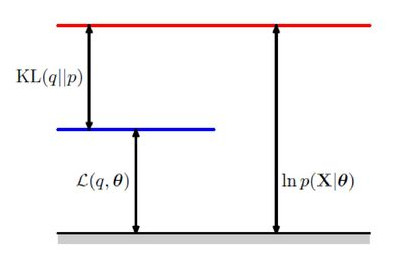
\includegraphics[width=0.4\textwidth]{fig/em-gap.jpg}
\end{figure}
\end{frame}

%%%%%%%%%%%%%%%%%%%%%%%%%%%%%%%%%%%%%%%%%%%%%%%%%%%%%%%%%%%%%%
\begin{frame}{Crucial point in ``Exact EM''}
 We \textbf{need} the exact a posteriori distribution: $p(\bs{z}|\bs{x};\bar{\bs{\Theta}})$.\vspace{3mm}
 
 What happens if we cannot use the exact posterior? \textbf{Approximate it}.\vspace{3mm}

 Two big families:
 \begin{itemize}
  \item $p(\bs{z}|\bs{x};\bar{\bs{\Theta}})$ has an analytic expression, but computationally too heavy.
  \item $p(\bs{z}|\bs{x};\bar{\bs{\Theta}})$ does not have an analytic expression.
 \end{itemize}\vspace{3mm}
 
 We will focus in the second case, and in a model called \textbf{Variational Autoencoders (VAE)}.
 

\end{frame}

% %%%%%%%%%%%%%%%%%%%%%%%%%%%%%%%%%%%%%%%%%%%%%%%%%%%%%%%%%%%%%%
% \begin{frame}{Example: switching linear dynamical system}
% \begin{columns}
%  \begin{column}{0.3\textwidth}
% \begin{figure}
%     \scalebox{0.7}{
%     \begin{tikzpicture}
%     \node[latent] (zm) {$\bs{z}_{t-1}$};
%     \node[latent,right=of zm] (z) {$\bs{z}_t$};
%     \node[latent,right=of z] (zp) {$\bs{z}_{t+1}$};
%     \path(zm) edge[->,blue] (z);
%     \path(z) edge[->,blue] (zp);
%     \onslide<2->{\node[latent,below=of zm] (ym) {$\bs{y}_{t-1}$};
%     \node[latent,below=of z,yshift=-1mm] (y) {$\bs{y}_t$};
%     \node[latent,below=of zp] (yp) {$\bs{y}_{t+1}$};
%     \path(ym) edge[->,red] (y);
%     \path(y) edge[->,red] (yp);
%     \path(zm) edge[->,red] (ym);
%     \path(z) edge[->,red] (y);
%     \path(zp) edge[->,red] (yp);
%     }
%     \onslide<3->{
%     \node[latent,below=of ym] (xm) {$\bs{x}_{t-1}$};
%     \node[latent,below=of y,yshift=-1mm] (x) {$\bs{x}_t$};
%     \node[latent,below=of yp] (xp) {$\bs{x}_{t+1}$};
%     \path(ym) edge[->,green] (xm);
%     \path(y) edge[->,green] (x);
%     \path(yp) edge[->,green] (xp);
%     \path(zm) edge [->,bend left,green] (xm);
%     \path(z) edge [->,bend left,green] (x);
%     \path(zp) edge [->,bend left,green] (xp);}
%     \end{tikzpicture}}
%   \end{figure}
%  \end{column}
%  \begin{column}{0.7\textwidth}
%  \small
%   \begin{equation}\bs{z}_t\in\{1,\ldots,K\}\qquad p(\bs{z}_1=k) = \pi_k,\end{equation}
%   \begin{equation}{\color{blue} p(\bs{z}_t=\ell|\bs{z}_{t-1}=k) = \tau_{k\ell}} \qquad \text{(``HMM'')}\end{equation}
%   \onslide<2->{\hrule\begin{equation}\bs{y}_t\in\mathbb{R}^{d_y}\quad p(\bs{y}_1|\bs{z}_1=k) = \MN(\bs{y}_1;\bs{a}_k,\bs{\Omega}_k)\end{equation}
%   \begin{equation}{\color{red}p(\bs{y}_t|\bs{y}_{t-1},\bs{z}_t=k) = \MN(\bs{y}_t;\bs{A}_k\bs{y}_{t-1},\bs{\Gamma}_k)}\quad \text{(``LDS'')}\end{equation}}
%   \onslide<3->{\hrule\begin{equation}\bs{x}_t\in\mathbb{R}^{d_x} \quad {\color{green}p(\bs{x}_t|\bs{y}_t,\bs{z}_t=k)=\MN(\bs{x}_t;\bs{C}_k\bs{y}_t,\bs{\Sigma}_k)}\end{equation}}
%  \end{column}
% \end{columns}
% \begin{itemize}
%  \item \textcolor{blue}{Discrete Markov chain} distribution on the $\bs{z}$'s.
%  \item<2-> \textcolor{red}{Continuous Markov chain} distribution on the $\bs{y}$'s conditioned by $\bs{z}$'s.
%  \item<3-> \textcolor{green}{Gaussian emission probability} on the $\bs{x}$ (conditioned by $\bs{y}$ and $\bs{z}$).
% \end{itemize}
% \end{frame}
% 
% %%%%%%%%%%%%%%%%%%%%%%%%%%%%%%%%%%%%%%%%%%%%%%%%%%%%%%%%%%%%%%
% \begin{frame}{The EM algorithm}
%  Let's derive the EM algorithm...\pause kidding (it's a good exercise!).\vspace{3mm}\\
%  
%  Even if there are two latent variables ($\bs{z}$ and $\bs{y}$), this model has the same structure of an HMM or an LDS (first-order Markovian dependencies on the latent variable). We will be needing a forward-backward!\vspace{3mm}\\
%  
%  For the forward, we need: $p(\bs{z}_t,\bs{y}_t,\bs{x}_{1:t})$ as a distribution on $(\bs{z}_t,\bs{y}_t)$.\\
%  Let's start for $t=1$:
%  \begin{align}
%   p(\bs{z}_1=k,\bs{y}_1,\bs{x}_{1}) = \MN(\bs{x}_1;\bs{C}_k\bs{y}_1,\bs{\Sigma}_k) \MN(\bs{y}_1;\bs{a}_k,\bs{\Omega}_k)\pi_k
%  \end{align}
%  This is a GMM with $K$ components. Nice!
%  \begin{equation}
%   \alpha_1(\bs{y}_1)=\sum_{k=1}^K p(\bs{z}_1=k,\bs{y}_1,\bs{x}_{1}) = \sum_{k=1}^K \MN(\bs{x}_1;\bs{C}_k\bs{y}_1,\bs{\Sigma}_k) \MN(\bs{y}_1;\bs{a}_k,\bs{\Omega}_k)\pi_k
%  \end{equation}
% 
% \end{frame}
% 
% %%%%%%%%%%%%%%%%%%%%%%%%%%%%%%%%%%%%%%%%%%%%%%%%%%%%%%%%%%%%%%
% \begin{frame}{The posterior distribution}
%  What about $t=2$?
%  \small
%  \begin{align}
%   &p(\bs{z}_2=\ell,\bs{y}_2,\bs{x}_{1:2}) = \sum_{k=1}^K \int p(\bs{z}_2=\ell,\bs{z}_1=k,\bs{y}_2,\bs{y}_1,\bs{x}_{1:2}) \textrm{d}\bs{y}_1 \\
%   &= \sum_{k=1}^K \int \MN(\bs{x}_2;\bs{C}_\ell\bs{y}_2,\bs{\Sigma}_\ell) \MN(\bs{y}_2;\bs{A}_\ell\bs{y}_1,\bs{\Gamma}_\ell) \tau_{k\ell} \MN(\bs{x}_1;\bs{C}_k\bs{y}_1,\bs{\Sigma}_k) \MN(\bs{y}_1;\bs{a}_k,\bs{\Omega}_k)\pi_k \textrm{d}\bs{y}_1\nonumber\\
%   &= \MN(\bs{x}_2;\bs{C}_\ell\bs{y}_2,\bs{\Sigma}_\ell) \sum_{k=1}^K \tau_{k\ell}\pi_k\int  \MN(\bs{y}_2;\bs{A}_\ell\bs{y}_1,\bs{\Gamma}_\ell)  \MN(\bs{x}_1;\bs{C}_k\bs{y}_1,\bs{\Sigma}_k) \MN(\bs{y}_1;\bs{a}_k,\bs{\Omega}_k) \textrm{d}\bs{y}_1 \nonumber
%  \end{align}
%  The integral is a Gaussian, and mutiplied with another Gaussian we obtain:
%  \begin{equation}
%   p(\bs{y}_2,\bs{x}_{1:2}) = \sum_{\ell=1}^K p(\bs{z}_2=\ell,\bs{y}_2,\bs{x}_{1:2})
%   = \sum_{\ell=1}^K\sum_{k=1}^K \MN(\bs{y}_2;\rule{4mm}{.5pt}_{k\ell},\rule{4mm}{.5pt}_{k\ell})
%  \end{equation}
%  This is a GMM with $K^2$ components!!!
% \end{frame}
% 
% %%%%%%%%%%%%%%%%%%%%%%%%%%%%%%%%%%%%%%%%%%%%%%%%%%%%%%%%%%%%%%
% \begin{frame}{The intractable posterior distribution}
%  You can easily prove now that:
%  \begin{equation}
%   p(\bs{y}_T,\bs{x}_{1:T}),
%  \end{equation}
% is a GMM with $K^T$ components.\vspace{3mm}\\
% 
% \begin{itemize}
%  \item Extermly slow since exponential in the sequence lenght.
%  \item Even if we had a supercomputer, we need the data!
% \end{itemize}\vspace{3mm}
% 
% The alternative is to approximate the distribution.
% 
% \end{frame}
% 
% %%%%%%%%%%%%%%%%%%%%%%%%%%%%%%%%%%%%%%%%%%%%%%%%%%%%%%%%%%%%%%
% \section{Variational Bayes Inference}
% %%%%%%%%%%%%%%%%%%%%%%%%%%%%%%%%%%%%%%%%%%%%%%%%%%%%%%%%%%%%%%
% 
% %%%%%%%%%%%%%%%%%%%%%%%%%%%%%%%%%%%%%%%%%%%%%%%%%%%%%%%%%%%%%%
% \begin{frame}{Intuition}
%  Find the ``best'' distribution within a family of distributions.\\ Like we do for function fitting:
%  \begin{figure}
%   \centering
%   \includegraphics[width=0.5\textwidth]{fig/function_approximation_1.png}
%  \end{figure}
%  In the figure the best function within a family (parabolae) is estimated.
% % \end{frame}
% 
% 
% 
% %%%%%%%%%%%%%%%%%%%%%%%%%%%%%%%%%%%%%%%%%%%%%%%%%%%%%%%%%%%%%%
% \begin{frame}{Approximating Family}
%  In VB inference, the approximate posterior is supposed to \textit{factorise}. For instance in the previous example:
%  \begin{figure}
%     \scalebox{0.7}{
%     \begin{tikzpicture}
%     \node[latent] (zm) {$\bs{z}_{t-1}$};
%     \node[latent,right=of zm] (z) {$\bs{z}_t$};
%     \node[latent,right=of z] (zp) {$\bs{z}_{t+1}$};
%     \path(zm) edge[->,blue] (z);
%     \path(z) edge[->,blue] (zp);
%     \node[latent,below=of zm] (ym) {$\bs{y}_{t-1}$};
%     \node[latent,below=of z,yshift=-1mm] (y) {$\bs{y}_t$};
%     \node[latent,below=of zp] (yp) {$\bs{y}_{t+1}$};
%     \path(ym) edge[->,red] (y);
%     \path(y) edge[->,red] (yp);
%     \path(zm) edge[->,red] (ym);
%     \path(z) edge[->,red] (y);
%     \path(zp) edge[->,red] (yp);
%     \node[latent,below=of ym] (xm) {$\bs{x}_{t-1}$};
%     \node[latent,below=of y,yshift=-1mm] (x) {$\bs{x}_t$};
%     \node[latent,below=of yp] (xp) {$\bs{x}_{t+1}$};
%     \path(ym) edge[->,green] (xm);
%     \path(y) edge[->,green] (x);
%     \path(yp) edge[->,green] (xp);
%     \path(zm) edge [->,bend left,green] (xm);
%     \path(z) edge [->,bend left,green] (x);
%     \path(zp) edge [->,bend left,green] (xp);
%     \end{tikzpicture}}
%   \end{figure}
%   We can approximate the exact posterior as:
%   \begin{equation}
%    p(\bs{y}_{1:T},\bs{z}_{1:T}|\bs{x}_{1:T}) \approx q(\bs{y}_{1:T},\bs{z}_{1:T}) = q_y(\bs{y}_{1:T})q_z(\bs{z}_{1:T}).
%   \end{equation}
% 
% \end{frame}
% 
% %%%%%%%%%%%%%%%%%%%%%%%%%%%%%%%%%%%%%%%%%%%%%%%%%%%%%%%%%%%%%%
% \begin{frame}{Approximating Criterion}
%  In which respect do we select the ``best'' distribution? Let's take a look back to the principle of the EM algorithm ($\bs{x}=\bs{x}_{1:T}$, same for $\bs{y}$ and $\bs{z}$):
%   \begin{align}
% \log p(\bs{x};\bs{\Theta}) &= \underbrace{\mathbb{E}_{q(\bs{y},\bs{z})}\Big\{\log \frac{p(\bs{x})p(\bs{y},\bs{z}|\bs{x})}{q(\bs{y},\bs{z})}\Big\}}_{\text{M-step}} +  \underbrace{D_{\text{KL}}\Big(q(\bs{y},\bs{z})\Big\lVert p(\bs{y},\bs{z}|\bs{x})\Big)}_{\text{E-step}}
% \end{align}\pause
% We should take the ``best'' in the Kullback-Leibler divergence sense:
% \begin{equation}
%  q_y^*,q_z^* = \arg\min_{q_y,q_z} D_{\text{KL}}\Big(q_y(\bs{y})q_z(\bs{z})\Big\lVert p(\bs{y},\bs{z}|\bs{x})\Big)
% \end{equation}
% \end{frame}
% 
% %%%%%%%%%%%%%%%%%%%%%%%%%%%%%%%%%%%%%%%%%%%%%%%%%%%%%%%%%%%%%%
% \begin{frame}{Solution}
%  By doing so we obtain the following optimal values:
%  \begin{equation}
%   q_y(\bs{y}) = \exp\left(\mathbb{E}_{q_z(\bs{z})}\{\log p(\bs{y},\bs{z}|\bs{x})\}\right)
%  \end{equation}
%  \begin{equation}
%    q_z(\bs{z}) = \exp\left(\mathbb{E}_{q_y(\bs{y})}\{\log p(\bs{y},\bs{z}|\bs{x})\}\right)
%  \end{equation}\vspace{3mm}\pause
%  
%  Therefore, the E-step requires to alternate between estimating $q_y$ and $q_z$. We refer to this as \textbf{variational expectation-maximisation} algorithm.\\
%  The M-step requires to compute:
%  \begin{equation}
%    \bs{\Theta}^* = \arg\max_{\bs{\Theta}} \mathbb{E}_{q_y(\bs{y})q_z(\bs{z})}\Big\{\log p(\bs{x},\bs{y},\bs{z};\bs{\Theta})\Big\}
%  \end{equation}
% 
% 
% \end{frame}
% %%%%%%%%%%%%%%%%%%%%%%%%%%%%%%%%%%%%%%%%%%%%%%%%%%%%%%%%%%%%%%
% \begin{frame}{General case}
%   In general, we can split the set of latent variables $\bs{H}$ into $M$ non-intersecting groups:
%   \begin{equation}
%    \bs{H} = \bs{H}_1\cup\ldots\cup\bs{H}_M.
%   \end{equation}\vspace{3mm}
%   
%   In that case the optimal E-step for $q_m(\bs{H}_m)$ requires the expectation w.r.t.\ to all other factors:
%    \begin{equation}
%    q_m(\bs{H}_m) = \exp\left(\mathbb{E}_{\prod_{k\neq m}q_k(\bs{H}_k)}\{\log p(\bs{H}|\bs{x})\}\right)
%  \end{equation}
% \end{frame}
% 
% %%%%%%%%%%%%%%%%%%%%%%%%%%%%%%%%%%%%%%%%%%%%%%%%%%%%%%%%%%%%%%
% \section{Variational Autoencoders}
% %%%%%%%%%%%%%%%%%%%%%%%%%%%%%%%%%%%%%%%%%%%%%%%%%%%%%%%%%%%%%%

%%%%%%%%%%%%%%%%%%%%%%%%%%%%%%%%%%%%%%%%%%%%%%%%%%%%%%%%%%%%%%
\begin{frame}{VAE Motivation: back to PPCA}
 Recall the definition of PPCA:
 \begin{itemize}
  \item $\bs{z}\sim\mathcal{N}(\bs{0},\bs{I})$,
  \item $\bs{x}|\bs{z}\sim\MN(\bs{x};\bs{A}\bs{z}+\bs{b},\sigma^2\bs{I})$, $\sigma>0$.
 \end{itemize}\vspace{3mm}
 
 Important limitations:
 \begin{itemize}
  \item The dependency of the mean with $\bs{z}$ is \textbf{afinne}.
  \item The covariance does not depend on $\bs{z}$.
 \end{itemize}\vspace{3mm}
 
 Non-linear generative model:
 \begin{itemize}
  \item $\bs{z}\sim\mathcal{N}(\bs{0},\bs{I})$,
  \item $\bs{x}|\bs{z}\sim\MN(\bs{x};\bs{\mu}_{\bs{\Theta}}(\bs{z}),\bs{\Sigma}_{\bs{\Theta}}(\bs{z}))$,
 \end{itemize}
 where $\bs{\mu}_{\bs{\Theta}}(\bs{z})$ and $\bs{\Sigma}_{\bs{\Theta}}(\bs{z})$ are (non-linear) functions parametrised by $\bs{\Theta}$.
\end{frame}


%%%%%%%%%%%%%%%%%%%%%%%%%%%%%%%%%%%%%%%%%%%%%%%%%%%%%%%%%%%%%%
\begin{frame}{Formalising the generative model (I)}
  The generative model:
 \begin{itemize}
  \item $\bs{z}\sim\mathcal{N}(\bs{0},\bs{I})$,
  \item $\bs{x}|\bs{z}\sim\MN(\bs{x};\bs{\mu}_{\bs{\Theta}}(\bs{z}),\bs{\Sigma}_{\bs{\Theta}}(\bs{z}))$,
 \end{itemize}
 where $\bs{\mu}_{\bs{\Theta}}(\bs{z})$ and $\bs{\Sigma}_{\bs{\Theta}}(\bs{z})$ will be implemented \textbf{by deep neural networks} parametrised by $\bs{\Theta}$ with input $\bs{z}$.\vspace{5mm}\pause
 
 A few comments:
 \begin{enumerate}
 \item The optimal parameters $\bs{\Theta}^*$ need to maximise the log-likelihood.
  %   We will be needing the posterior distribution $p(\bs{z}|\bs{x})$.
  \item $\bs{\Theta}$ cannot be estimated in closed-form.
  \item $\bs{\mu}_{\bs{\Theta}}(\bs{z})$ and $\bs{\Sigma}_{\bs{\Theta}}(\bs{z})$ are differentiable w.r.t.\ $\bs{\Theta}$, and $\bs{z}$.
  \item $\bs{\Sigma}_{\bs{\Theta}}(\bs{z})$ needs to be a covariance matrix.
 \end{enumerate}

\end{frame}

%%%%%%%%%%%%%%%%%%%%%%%%%%%%%%%%%%%%%%%%%%%%%%%%%%%%%%%%%%%%%%
\begin{frame}{Formalising the generative model (II)}
  How can we ensure that $\bs{\Sigma}_{\bs{\Theta}}(\bs{z})$ is a covariance matrix?
  \begin{itemize}
   \item The covariance matrix is assumed to be diagonal:
   \begin{equation}\bs{\Sigma}_{\bs{\Theta}}(\bs{z}) = \left(\begin{array}{cccc} 
   \nu^{(1)}_{\bs{\Theta}}(\bs{z}) & 0 & \cdots & 0 \\ 
   0 & \nu^{(2)}_{\bs{\Theta}}(\bs{z}) & \cdots & 0 \\
   \vdots & \vdots & \ddots & \vdots \\
   0 & 0 & \cdots & \nu^{(D)}_{\bs{\Theta}}(\bs{z})
   \end{array}\right)\end{equation}
   Reduces complexity and memory, but also expressivity.
   \item We estimate the log-variance: $\eta^{(d)}_{\bs{\Theta}}(\bs{z}) = \log \nu^{(d)}_{\bs{\Theta}}(\bs{z})$:
   \begin{equation}\bs{\Sigma}_{\bs{\Theta}}(\bs{z}) = \textrm{diag}_d \left(\exp \left(\eta^{(d)}_{\bs{\Theta}}(\bs{z})\right)\right)\end{equation}
   The values of $\eta^{(d)}_{\bs{\Theta}}(\bs{z})$ can be positive or negative.
  \end{itemize}
  

\end{frame}

%%%%%%%%%%%%%%%%%%%%%%%%%%%%%%%%%%%%%%%%%%%%%%%%%%%%%%%%%%%%%%
\begin{frame}{Formalising the generative model (III)}
  In terms of probabilistic dependencies, they are the same as PPCA:\vspace{3mm}\\
  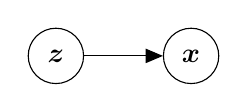
\begin{tikzpicture}[->]
   \node[latent,draw] (z)  {$\bs{z}$};
   \node[latent,draw,right=of z] (x) {$\bs{x}$};
   \edge{z} {x};
  \end{tikzpicture}\vspace{3mm}

  But I would like to draw also the non-lineariry:\vspace{3mm}
  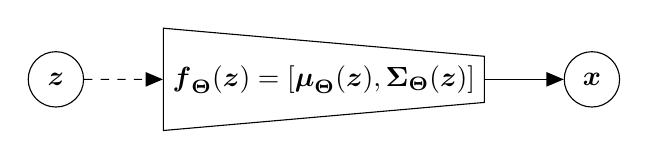
\begin{tikzpicture}[->]
   \node[latent,draw] (z)  {$\bs{z}$};
   \node[net,draw,trapezium angle=85,right=of z] (dec) {$\bs{f}_{\bs{\Theta}}(\bs{z})=[\bs{\mu}_{\bs{\Theta}}(\bs{z}),\bs{\Sigma}_{\bs{\Theta}}(\bs{z})]$};
   \node[latent,draw,right=of dec] (x) {$\bs{x}$};
   \edge[dashed] {z} {dec};
   \edge{dec} {x};
  \end{tikzpicture}\vspace{3mm}
  
  The dependency of the parameters w.r.t.\ $\bs{z}$ is \textbf{deterministic}.\vspace{3mm}
  
  Denoted by $\bs{f}_{\bs{\Theta}}(\bs{z}):\mathbb{R}^{d_z}\rightarrow\mathbb{R}^{2d_x}$, this non-linearity is implemented with a deep network, with parameters (weights and biases) $\bs{\Theta}$.

\end{frame}

%%%%%%%%%%%%%%%%%%%%%%%%%%%%%%%%%%%%%%%%%%%%%%%%%%%%%%%%%%%%%%
\begin{frame}{The posterior distribution}
 For any EM-like procedure, we would need the posterior distribution:
 \begin{align}
  p(\bs{z}|\bs{x}) & \stackrel{(\bs{z})}{\propto}  p(\bs{x}|\bs{z})p(\bs{z}) \\
  &\stackrel{(\bs{z})}{\propto} \MN(\bs{x};\bs{\mu}_{\bs{\Theta}}(\bs{z}),\bs{\Sigma}_{\bs{\Theta}}(\bs{z})) \MN(\bs{z};\bs{0},\bs{I}) \\
  &\stackrel{(\bs{z})}{\propto} \frac{1}{|\bs{\Sigma}_{\bs{\Theta}}(\bs{z})|^{1/2}} \exp\left(-\frac{1}{2} (\bs{x}-\bs{\mu}_{\bs{\Theta}}(\bs{z}))^\top \bs{\Sigma}_{\bs{\Theta}}^{-1}(\bs{z})(\bs{x}-\bs{\mu}_{\bs{\Theta}}(\bs{z})) - \frac{1}{2}\lVert\bs{z}\rVert^2 \right)
 \end{align}\pause
 
 We cannot go our ``standard'' way, because we cannot identify a distribution on $\bs{z}$.\vspace{3mm}
 
 The posterior distribution cannot be computed analytically!!!

\end{frame}

%%%%%%%%%%%%%%%%%%%%%%%%%%%%%%%%%%%%%%%%%%%%%%%%%%%%%%%%%%%%%%
\begin{frame}{Approximating the posterior distribution (I)}
 The posterior distribution needs to be approximated. We will propose a family of distributions, and find the \textbf{\textcolor{blue}{best candidate within this family}}.\vspace{3mm}\\
 
 \begin{figure}
  \centering
  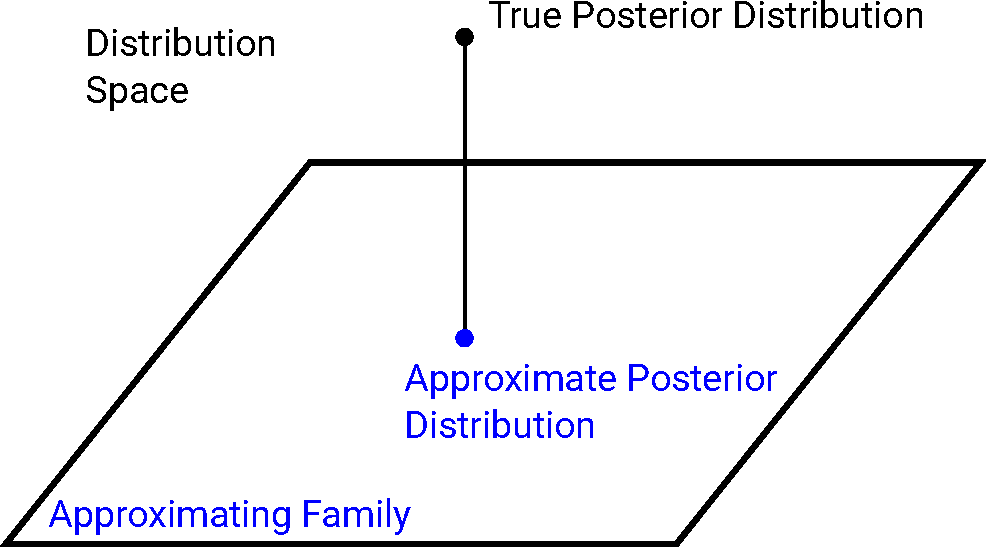
\includegraphics[width=0.6\textwidth]{fig/distribution_projection.pdf}
 \end{figure}

\end{frame}

%%%%%%%%%%%%%%%%%%%%%%%%%%%%%%%%%%%%%%%%%%%%%%%%%%%%%%%%%%%%%%
\begin{frame}{Approximating the posterior distribution (II)}

 The posterior distribution will be approximated with \textbf{another} feed-forward network parametrised with $\bs{\Phi}$:
 \begin{equation}p(\bs{z}|\bs{x})\approx q(\bs{z}|\bs{x}) = \MN(\bs{z};\tilde{\bs{\mu}}_{\bs{\Phi}}(\bs{x}),\tilde{\bs{\Sigma}}_{\bs{\Phi}}(\bs{x}))\end{equation}
 
 The approximating family is composed of all the distributions that can be expressed as above, for a certain value of $\bs{\Phi}$.
 \begin{equation}\mathcal{G} = \{ \bs{g}_{\bs{\Phi}}:\mathbb{R}^{d_x}\rightarrow\mathbb{R}^{2d_z};\bs{\Phi}\in\bs{\Phi} \},\end{equation}
 with $\bs{g}_{\bs{\Phi}}(\bs{x}) = [\tilde{\bs{\mu}}_{\bs{\Phi}}(\bs{x}),\tilde{\bs{\Sigma}}_{\bs{\Phi}}(\bs{x})]$.
\end{frame}

%%%%%%%%%%%%%%%%%%%%%%%%%%%%%%%%%%%%%%%%%%%%%%%%%%%%%%%%%%%%%%
\begin{frame}{Overall architecture}
 If we ``chain'' the posterior and the generative model:\vspace{3mm}
   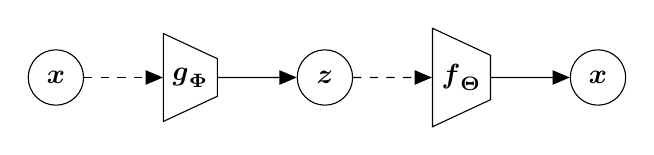
\begin{tikzpicture}[->]
   \node[latent,draw] (xi) {$\bs{x}$};
   \node[net,draw,right=of xi] (enc) {$\bs{g}_{\bs{\Phi}}$};
   \node[latent,draw,right=of enc] (z)  {$\bs{z}$};
   \node[net,draw,right=of z] (dec) {$\bs{f}_{\bs{\Theta}}$};
   \node[latent,draw,right=of dec] (x) {$\bs{x}$};
   \edge[dashed] {xi} {enc};
   \edge{enc} {z};
   \edge[dashed] {z} {dec};
   \edge{dec} {x};
  \end{tikzpicture}\vspace{3mm}
 
 \begin{itemize}
  \item The generative model is also called the \textbf{decoder}.
  \item The inference or posterior is also called the \textbf{encoder}.
 \end{itemize}\vspace{3mm}
 
 This is why we call these architectures \textbf{variational autoencoders} VAE.\vspace{3mm}
 
 But how do we optimise for the parameters $\bs{\Theta}$ and $\bs{\Phi}$?

\end{frame}

%%%%%%%%%%%%%%%%%%%%%%%%%%%%%%%%%%%%%%%%%%%%%%%%%%%%%%%%%%%%%%
\begin{frame}{Learning - ELBO}
 If we recall the formulation for the EM:
 \begin{align}
\log p(\bs{x}) &= \mathbb{E}_{q(\bs{z}|\bs{x})}\Big\{\log \frac{p(\bs{x},\bs{z})}{q(\bs{z}|\bs{x})}\Big\} + {\color{green} D_{\text{KL}}\Big(q(\bs{z}|\bs{x})\Big\lVert p(\bs{z}|\bs{x})\Big)}
\end{align}
Problem: the second term cannot be computed! But it's positive:
 \begin{align}
\log p(\bs{x};\bs{\Theta},\bs{\Phi}) &\; {\color{green}\geq}\; {\color{blue} \mathbb{E}_{q_{\bs{\Phi}}(\bs{z}|\bs{x})}\Big\{\log \frac{p(\bs{x},\bs{z})}{q_{\bs{\Phi}}(\bs{z}|\bs{x})}\Big\}} \\
\log p(\bs{x};\bs{\Theta},\bs{\Phi}) &\; {\color{green}\geq}\; {\color{blue} \underbrace{\mathbb{E}_{q_{\bs{\Phi}}(\bs{z}|\bs{x})}\Big\{\log p_{\bs{\Theta}}(\bs{x}|\bs{z})\Big\}}_{\text{Reconstruction}} -  \underbrace{D_{\text{KL}}\Big(q_{\bs{\Phi}}(\bs{z}|\bs{x})\Big\lVert p(\bs{z})\Big)}_{\text{Regularisation}}}
\end{align}
This is known as \textbf{Evidence Lower-BOund or ELBO}: $\mathcal{L}_{\text{ELBO}}(\bs{\Theta},\bs{\Phi})$.\vspace{3mm}\\
Be VERY careful with these expressions.\\ They look alike, but they are NOT the same.
\end{frame}

%%%%%%%%%%%%%%%%%%%%%%%%%%%%%%%%%%%%%%%%%%%%%%%%%%%%%%%%%%%%%%
\begin{frame}{Learning - Sampling}
 But we still have one problem:
 \begin{align}
  \mathcal{L}_{\text{ELBO}}(\bs{\Theta},\bs{\Phi}) &= \underbrace{\mathbb{E}_{q_{\bs{\Phi}}(\bs{z}|\bs{x})}\Big\{\log p_{\bs{\Theta}}(\bs{x}|\bs{z})\Big\}}_{\text{Reconstruction}} -  \underbrace{D_{\text{KL}}\Big(q_{\bs{\Phi}}(\bs{z}|\bs{x})\Big\lVert p(\bs{z})\Big)}_{\text{Regularisation}}
\end{align}
To compute the ``reconstruction'' term we need to take the expectation w.r.t.\ $q_{\bs{\Phi}}(\bs{z}|\bs{x})$, but recall that:
\begin{equation}
  p_{\bs{\Theta}}(\bs{x}|\bs{z}) = \MN(\bs{x};\bs{\mu}_{\bs{\Theta}}(\bs{z}),\bs{\Sigma}_{\bs{\Theta}}(\bs{z})).
\end{equation}
Due to the non-linearity, we cannot compute the reconstruction term in closed form $\rightarrow$ we sample $R$ points $\hat{\bs{z}}_1,\ldots,\hat{\bs{z}}_R$ from $q_{\bs{\Phi}}$:
 \begin{align}
  \mathcal{L}_{\text{ELBO}}(\bs{\Theta},\bs{\Phi}) &= \underbrace{\frac{1}{R}\sum_{r=1}^R\log p_{\bs{\Theta}}(\bs{x}|\hat{\bs{z}}_r)}_{\text{Reconstruction}} -  \underbrace{D_{\text{KL}}\Big(q_{\bs{\Phi}}(\bs{z}|\bs{x})\Big\lVert p(\bs{z})\Big)}_{\text{Regularisation}}
\end{align}
\end{frame}

%%%%%%%%%%%%%%%%%%%%%%%%%%%%%%%%%%%%%%%%%%%%%%%%%%%%%%%%%%%%%%
\begin{frame}{Learning - Gradient ascent?}
  Let's go back to the architecture:\vspace{3mm}
   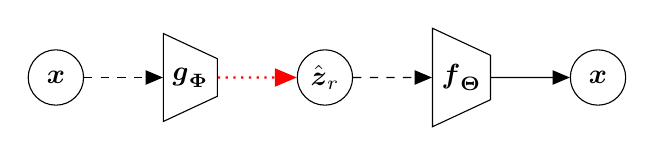
\begin{tikzpicture}[->]
   \node[latent,draw] (xi) {$\bs{x}$};
   \node[net,draw,right=of xi] (enc) {$\bs{g}_{\bs{\Phi}}$};
   \node[latent,draw,right=of enc] (z)  {$\hat{\bs{z}}_r$};
   \node[net,draw,right=of z] (dec) {$\bs{f}_{\bs{\Theta}}$};
   \node[latent,draw,right=of dec] (x) {$\bs{x}$};
   \edge[dashed] {xi} {enc};
   \edge[dotted,thick,red] {enc} {z};
   \edge[dashed] {z} {dec};
   \edge{dec} {x};
  \end{tikzpicture}\\
  where dashed lines are deterministic, dotted lines are sampling\\ (we will see later for the solid line).\vspace{3mm}
  
  We agreed that there is no closed-form solution for the parameters (due to non-linearity). We will learn the parameters using stochastic gradient ascent (to maximise the ELBO).\vspace{3mm}
  
  We assume that $\bs{g}_{\bs{\Phi}}$ and $\bs{f}_{\bs{\Theta}}$ are differentiable (to compute the gradient).\vspace{3mm}
  
  The sampling operation from $q_{\bs{\Phi}}$ is {\color{red}NOT} differentiable w.r.t.\ $\bs{\Phi}$.
\end{frame}

%%%%%%%%%%%%%%%%%%%%%%%%%%%%%%%%%%%%%%%%%%%%%%%%%%%%%%%%%%%%%%
\begin{frame}{Learning - Reparametrisation trick}
 We use the so-called \textbf{reparametrisation trick}:\vspace{3mm}
    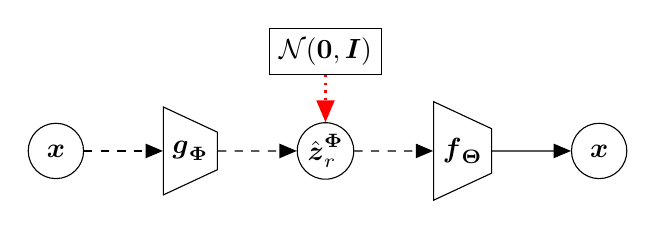
\begin{tikzpicture}[->]
   \node[latent,draw] (xi) {$\bs{x}$};
   \node[net,draw,right=of xi] (enc) {$\bs{g}_{\bs{\Phi}}$};
   \node[latent,draw,right=of enc] (z)  {$\hat{\bs{z}}_r^{\bs{\Phi}}$};
   \node[net,draw,right=of z] (dec) {$\bs{f}_{\bs{\Theta}}$};
   \node[latent,draw,right=of dec] (x) {$\bs{x}$};
   \node[draw,above=of z,yshift=-4mm] (standard) {$\MN(\bs{0},\bs{I})$};
   \edge[dashed] {xi} {enc};
   \edge[dashed] {enc} {z};
   \edge[dotted,thick,red] {standard} {z};
   \edge[dashed] {z} {dec};
   \edge{dec} {x};
  \end{tikzpicture}\vspace{3mm}\\
  Formally ($\hat{\bs{z}}_r^{\bs{\Phi}}$ denotes explicitly the dependency on $\bs{\Phi}$):
  \begin{equation}
   \hat{\bs{z}}_r^{\bs{\Phi}} = \tilde{\bs{\Sigma}}_{\bs{\Phi}}^{1/2}\hat{\bs{\epsilon}}_r + \tilde{\bs{\mu}}_{\bs{\Phi}} \quad\text{with}\quad \hat{\bs{\epsilon}}_r\sim \MN(\bs{0},\bs{I})
  \end{equation}
  So we sample from a standard Gaussian, and use the parameters $ \tilde{\bs{\mu}}_{\bs{\Phi}}$ and $\tilde{\bs{\Sigma}}_{\bs{\Phi}} $ in \textbf{differentiable operations} (multiplication and addition).\vspace{3mm}\\
  
  If the last arrow is differentiable, then we can use gradient ascent.
\end{frame}

%%%%%%%%%%%%%%%%%%%%%%%%%%%%%%%%%%%%%%%%%%%%%%%%%%%%%%%%%%%%%%
\begin{frame}{Learning - Reparametrisation trick (II)}
 Another way to see the reparametrisation trick (from ``An Introduction to Variational Autoencoders'' by Diederik P. Kingma, Max Welling, \texttt{chamilo}):\\
 \centering
 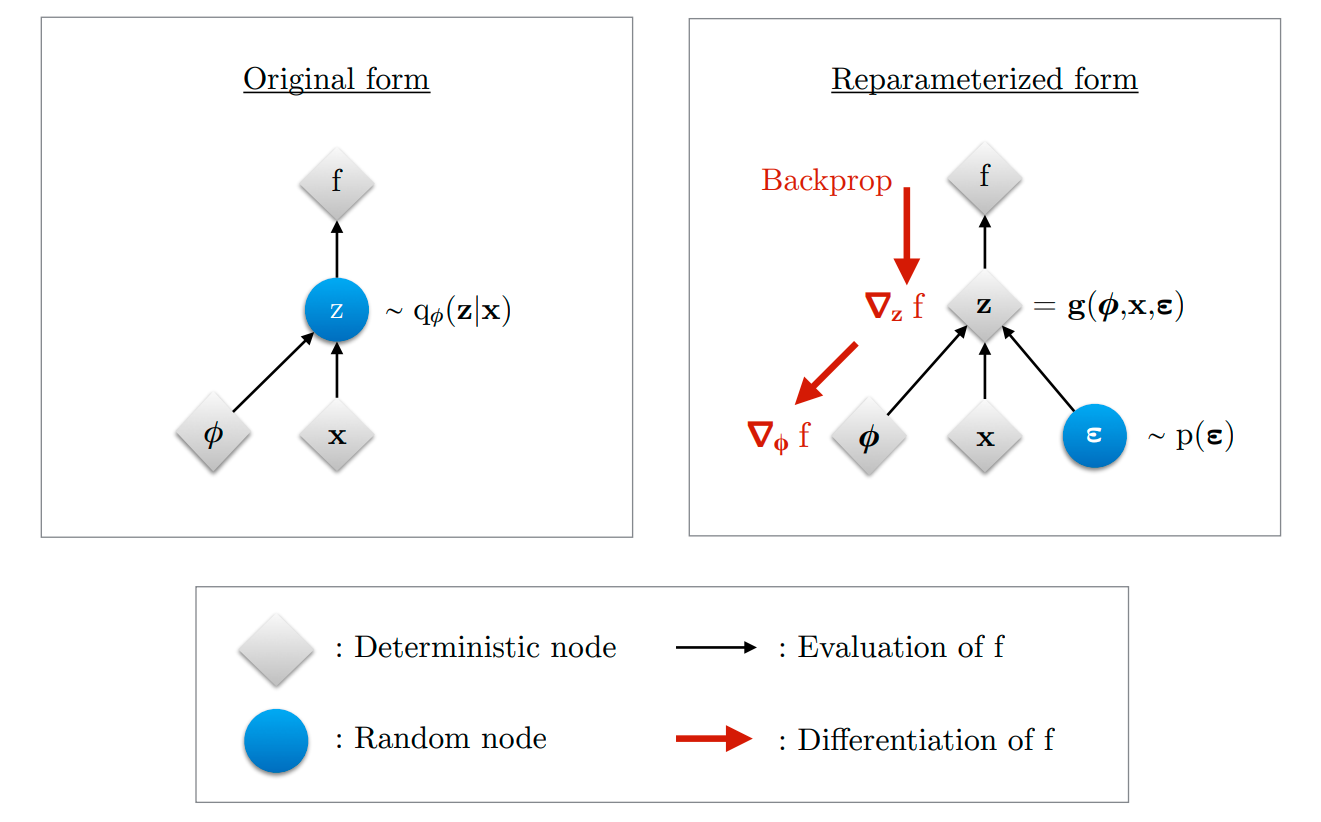
\includegraphics[width=0.9\textwidth]{fig/reparametrisationtrick.png}
\end{frame}

%%%%%%%%%%%%%%%%%%%%%%%%%%%%%%%%%%%%%%%%%%%%%%%%%%%%%%%%%%%%%%
\begin{frame}{Learning - The loss}
We are now ready to write the loss:
\begin{align}
 \mathcal{L}_{\text{ELBO}}(\bs{\Theta},\bs{\Phi}) &= \underbrace{\mathbb{E}_{q_{\bs{\Phi}}(\bs{z}|\bs{x})}\Big\{\log p_{\bs{\Theta}}(\bs{x}|\bs{z})\Big\}}_{\text{Reconstruction}} -  \underbrace{D_{\text{KL}}\Big(q_{\bs{\Phi}}(\bs{z}|\bs{x})\Big\lVert p(\bs{z})\Big)}_{\text{Regularisation}}\\
 &= \underbrace{\sum_{r=1}^R\log p_{\bs{\Theta}}(\bs{x}|\hat{\bs{z}}_r^{\bs{\Phi}})}_{\text{Reconstruction}} -  \underbrace{D_{\text{KL}}\Big(q_{\bs{\Phi}}(\bs{z}|\bs{x})\Big\lVert p(\bs{z})\Big)}_{\text{Regularisation}} \\
 &\stackrel{(\bs{\Theta},\bs{\Phi})}{=} -\frac{1}{2}\Bigg[\frac{1}{R}\sum_{r=1}^R \left(\log \lvert \bs{\Sigma}_{\bs{\Theta}}(\hat{\bs{z}}_r^{\bs{\Phi}})\rvert + \lVert \bs{x}-\bs{\mu}_{\bs{\Theta}}(\hat{\bs{z}}_r^{\bs{\Phi}})\rVert^2_{\bs{\Sigma}_{\bs{\Theta}}(\hat{\bs{z}}_r^{\bs{\Phi}})} \right)\label{eq:recon}\\
 &\phantom{\stackrel{(\bs{\Theta},\bs{\Phi})}{=} -\frac{1}{2}\Bigg[}+\textrm{Tr}(\bs{\Sigma}_{\bs{\Phi}}(\bs{x})) + \lVert\bs{\mu}_{\bs{\Phi}}(\bs{x})\rVert^2 - \log \lvert\bs{\Sigma}_{\bs{\Phi}}(\bs{x})\rvert\Bigg]\label{eq:reg}
\end{align}
Where~(\ref{eq:recon}) and~(\ref{eq:reg}) are the reconstruction and regularisation terms resp.\\
\textbf{Homework}: use the definition of the terms above to prove that.
\end{frame}

%%%%%%%%%%%%%%%%%%%%%%%%%%%%%%%%%%%%%%%%%%%%%%%%%%%%%%%%%%%%%%
\begin{frame}{Learning - The loss (II)}
 \begin{align}
 \mathcal{L}_{\text{ELBO}}(\bs{\Theta},\bs{\Phi}) &\stackrel{(\bs{\Theta},\bs{\Phi})}{=} -\frac{1}{2}\Bigg[\frac{1}{R}\sum_{r=1}^R \left(\log \lvert \bs{\Sigma}_{\bs{\Theta}}(\hat{\bs{z}}_r^{\bs{\Phi}})\rvert + {\color{blue}\lVert \bs{x}-\bs{\mu}_{\bs{\Theta}}(\hat{\bs{z}}_r^{\bs{\Phi}})\rVert^2_{\bs{\Sigma}_{\bs{\Theta}}(\hat{\bs{z}}_r^{\bs{\Phi}})}}\right)\\
 &\phantom{\stackrel{(\bs{\Theta},\bs{\Phi})}{=} -\frac{1}{2}\Bigg[}+\textrm{Tr}(\bs{\Sigma}_{\bs{\Phi}}(\bs{x})) + \lVert\bs{\mu}_{\bs{\Phi}}(\bs{x})\rVert^2 - \log \lvert\bs{\Sigma}_{\bs{\Phi}}(\bs{x})\rvert\Bigg]
\end{align}
Comments:
\begin{itemize}
 \item We recall that $ \hat{\bs{z}}_r^{\bs{\Phi}} = \tilde{\bs{\Sigma}}_{\bs{\Phi}}^{1/2}\hat{\bs{\epsilon}}_r + \tilde{\bs{\mu}}_{\bs{\Phi}} $ with $\hat{\bs{\epsilon}}_r\sim \MN(\bs{0},\bs{I})$.
 \item We remark that all operators are differentiable w.r.t.\ $\bs{\Theta}$ and $\bs{\Phi}$.
 \item If we remove the ``$-\frac{1}{2}$'' we use gradient descent.
 \item The term in blue is the {\color{blue}Mahalanobis distance} and can be replaced...
\end{itemize}

\end{frame}

%%%%%%%%%%%%%%%%%%%%%%%%%%%%%%%%%%%%%%%%%%%%%%%%%%%%%%%%%%%%%%
\begin{frame}{Other reconstruction losses}
 Often, we forget about the covariance matrix of the generative model $\bs{\Sigma}_{\bs{\Theta}}$ and use other distances rather than Mahalanobis:
 \begin{itemize}
  \item The Euclidean distance (equivalent to set $\bs{\Sigma}_{\bs{\Theta}}=\bs{I}$): $\lVert \bs{x}-\bs{\mu}_{\bs{\Theta}}(\hat{\bs{z}}_r^{\bs{\Phi}})\rVert^2_2$
  \item The $L_1$ distance: $\lVert \bs{x}-\bs{\mu}_{\bs{\Theta}}(\hat{\bs{z}}_r^{\bs{\Phi}})\rVert_1$ (links with the Laplace distribution)
 \end{itemize}

 In these cases $\bs{f}_{\bs{\Theta}}(\bs{z}):\mathbb{R}^{d_z}\rightarrow\mathbb{R}^{d_x}$ (instead of $\mathbb{R}^{2d_x}$), and this links to the deterministic autoencoders.\vspace{6mm}
 
 In addition, we can attempt to reconstruct $\bs{x}$ from another signal $\tilde{\bs{x}}$:
 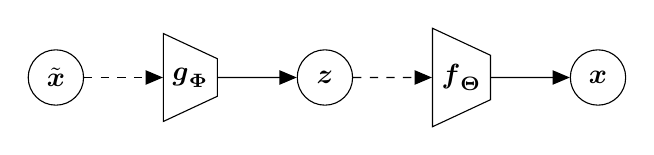
\begin{tikzpicture}[->]
   \node[latent,draw] (xi) {$\tilde{\bs{x}}$};
   \node[net,draw,right=of xi] (enc) {$\bs{g}_{\bs{\Phi}}$};
   \node[latent,draw,right=of enc] (z)  {$\bs{z}$};
   \node[net,draw,right=of z] (dec) {$\bs{f}_{\bs{\Theta}}$};
   \node[latent,draw,right=of dec] (x) {$\bs{x}$};
   \edge[dashed] {xi} {enc};
   \edge{enc} {z};
   \edge[dashed] {z} {dec};
   \edge{dec} {x};
  \end{tikzpicture}\\
 a clear example are denoising VAE ($\tilde{\bs{x}}=\bs{x}+\bs{b}$, with $\bs{b}$ being noise).\vspace{-3mm}
\end{frame}

%%%%%%%%%%%%%%%%%%%%%%%%%%%%%%%%%%%%%%%%%%%%%%%%%%%%%%%%%%%%%%
\begin{frame}{Differences w.r.t.\ EM}
\textbf{[EM]}: Start with $\bar{\bs{\Theta}}$:
\begin{itemize}
 \item E-step: Compute $p(\bs{z}_n|\bs{x}_n;\bar{\bs{\Theta}})$, $\forall n$.
 \item M-step: Compute $\bs{\Theta}^*$, and set $\bar{\bs{\Theta}}$ to that.
\end{itemize}
(Until convergence)\vspace{5mm}\\

\textbf{[SGD]}: Start with $\bar{\bs{\Theta}}$. Initialise also $\bar{\bs{\Phi}}$:
\begin{itemize}
 \item Forward: Compute $\bs{g}_{\bar{\bs{\Phi}}}(\bs{x}_n)$, sample $\bs{z}_n$, compute $\bs{f}_{\bar{\bs{\Theta}}}(\bs{z}_n)$, $\forall n$ in batch.
 \item Backward: Compute $\mathcal{L}_{\text{ELBO}}$, $\nabla_{\bar{\bs{\Theta}}}\mathcal{L}_{\text{ELBO}}$, and $\nabla_{\bar{\bs{\Phi}}}\mathcal{L}_{\text{ELBO}}$.
 \item Update $\bar{\bs{\Theta}}$ and $\bar{\bs{\Phi}}$ with your preferred gradient update rule.
\end{itemize}
(Until convergence)\\
 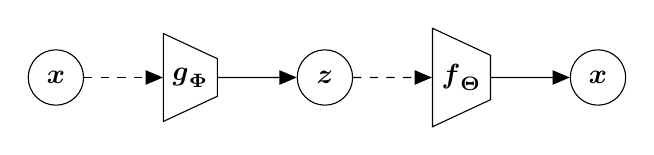
\begin{tikzpicture}[->]
   \node[latent,draw] (xi) {$\bs{x}$};
   \node[net,draw,right=of xi] (enc) {$\bs{g}_{\bs{\Phi}}$};
   \node[latent,draw,right=of enc] (z)  {$\bs{z}$};
   \node[net,draw,right=of z] (dec) {$\bs{f}_{\bs{\Theta}}$};
   \node[latent,draw,right=of dec] (x) {$\bs{x}$};
   \edge[dashed] {xi} {enc};
   \edge{enc} {z};
   \edge[dashed] {z} {dec};
   \edge{dec} {x};
  \end{tikzpicture}
\end{frame}

%%%%%%%%%%%%%%%%%%%%%%%%%%%%%%%%%%%%%%%%%%%%%%%%%%%%%%%%%%%%%%
\begin{frame}{VAE Summary}
 The models ($\bs{\Theta}$ and $\bs{\Phi}$ are the parameters of the respective networks):
\begin{itemize}
\item \textbf{Gen/dec}: $p(\bs{x}|\bs{z})=\MN(\bs{x};\bs{\mu}_{\bs{\Theta}}(\bs{z}),\bs{\Sigma}_{\bs{\Theta}}(\bs{z}))$, $p(\bs{z})=\mathcal{N}(\bs{0},\bs{I})$
\item \textbf{Inf/enc}: $p(\bs{z}|\bs{x})\approx q(\bs{z}|\bs{x}) = \MN(\bs{z};\tilde{\bs{\mu}}_{\bs{\Phi}}(\bs{x}),\tilde{\bs{\Sigma}}_{\bs{\Phi}}(\bs{x}))$
\end{itemize}\vspace{3mm}

The loss (\textbf{ELBO}) needs \textbf{sampling}, $\hat{\bs{z}}_1,\ldots,\hat{\bs{z}}_R \sim q_{\bs{\Phi}}$:
\begin{align}
  \mathcal{L}_{\text{ELBO}}(\bs{\Theta},\bs{\Phi}) &= \underbrace{\frac{1}{R}\sum_{r=1}^R\log p_{\bs{\Theta}}(\bs{x}|\hat{\bs{z}}_r)}_{\text{Reconstruction}} -  \underbrace{D_{\text{KL}}\Big(q_{\bs{\Phi}}(\bs{z}|\bs{x})\Big\lVert p(\bs{z})\Big)}_{\text{Regularisation}}
\end{align}
 We use the \textbf{reparametrisation trick}: $\hat{\bs{z}}_r^{\bs{\Phi}} = \tilde{\bs{\Sigma}}_{\bs{\Phi}}^{1/2}\hat{\bs{\epsilon}}_r + \tilde{\bs{\mu}}_{\bs{\Phi}}, \hat{\bs{\epsilon}}_r\sim \MN(\bs{0},\bs{I})$\vspace{3mm}
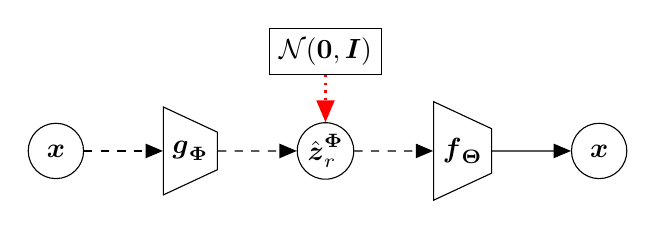
\begin{tikzpicture}[->]
   \node[latent,draw] (xi) {$\bs{x}$};
   \node[net,draw,right=of xi] (enc) {$\bs{g}_{\bs{\Phi}}$};
   \node[latent,draw,right=of enc] (z)  {$\hat{\bs{z}}_r^{\bs{\Phi}}$};
   \node[net,draw,right=of z] (dec) {$\bs{f}_{\bs{\Theta}}$};
   \node[latent,draw,right=of dec] (x) {$\bs{x}$};
   \node[draw,above=of z,yshift=-4mm] (standard) {$\MN(\bs{0},\bs{I})$};
   \edge[dashed] {xi} {enc};
   \edge[dashed] {enc} {z};
   \edge[dotted,thick,red] {standard} {z};
   \edge[dashed] {z} {dec};
   \edge{dec} {x};
\end{tikzpicture}
\end{frame}

\end{document}



